\section{Results}
\label{sec:results}

\subsection{Machine Learning}
\label{sec:learning}

We used the training data of 20 different projects on three commonly used machine learning algorithms.
The projects varied in size and the algorithms we tested are: Logistic Regression, Naive Bayes and Random Forest.
We ran the algorithm against each of the 20 projects with a 10-fold cross-validation.
The models were trained with 90\% of the training data, the remaining 10\% was used as test data.

In table~\ref{tab:alg-compare} it can be seen how the three algorithms performed on average.
Both LR and NB perform well on recall, but have a very low precision which makes it unusable for our application.
The RF algorithm performs less on recall, but achieves a higher precision, which is more important in our case.
High precision means that the algorithm returned substantially more relevant results than irrelevant.
It seems that RF is the best at identifying the important pull requests.

\begin{table}
  \begin{tabular}{ l | c | c | c | c | c | c }
    Alg. & $\overline{p}$ & $\sigma(p)$ & $\overline{r}$ & $\sigma(r)$ & $\overline{F1}$ & $\sigma(F1)$ \\ \hline
    \hline
    LR & .2423 & .1721 & .8377 & .0581 & .3455 & .1925 \\ \hline
    NB & .2219 & .1527 & .8048 & .0704 & .3198 & .1718 \\ \hline
    RF & .6885 & .1120 & .4979 & .1270 & .5715 & .1157 \\
  \end{tabular}
  \caption[Comparision of algorithms]{Comparision of algorithms. The average precision, recall and F1-score for each algorithm. }
  \label{tab:alg-compare}
\end{table}

The results in table~\ref{tab:alg-compare} led us believe that there was room for improvement.
Since the important snapshot data vs. unimportant data is very imbalanced, we decided to tune the balance.
By restricting the number of unimportant snapshots (F) to a multiple of the important part (T) we obtained the averaged results in table~\ref{tab:balance}.
The four different balanced ratios were applied in 10-fold for each project.

\begin{table}
  \begin{tabular}{ l | c | c | c | c | c | c }
    F:T & $\overline{p}$ & $\sigma(p)$ & $\overline{r}$ & $\sigma(r)$ & $\overline{F1}$ & $\sigma(F1)$ \\ \hline
    \hline
    4F:1T & .6001 & .1676 & .5769 & .1047 & .5721 & .1141 \\ \hline
    3F:1T & .5674 & .1787 & .6015 & .0939 & .5658 & .1206 \\ \hline
    2F:1T & .5235 & .1965 & .6549 & .0945 & .5564 & .1475 \\ \hline
    1F:1T & .4586 & .2450 & .7630 & .0600 & .5376 & .2030 \\
  \end{tabular}
  \caption[Comparision of balanced data]{Comparision of balanced data. The average precision, recall and F1-score for each balanced set. }
  \label{tab:balance}
\end{table}

Balancing the data turned out to make things worse.
Only when the unimportant part is four times larger than the important part the performance is the same as the unbalanced data.

Our last attempt to improve the performance was to a different feature selection.
A feature importance plot of one of the projects is shown in figure~\ref{fig:feature-importance}.
It shows very clear that the age is the dominant factor for the prediction model.
This is true for almost all our selected projects.
Based on this information we decided to see what happens if we disabled the age feature.

\begin{figure}
  \centering
  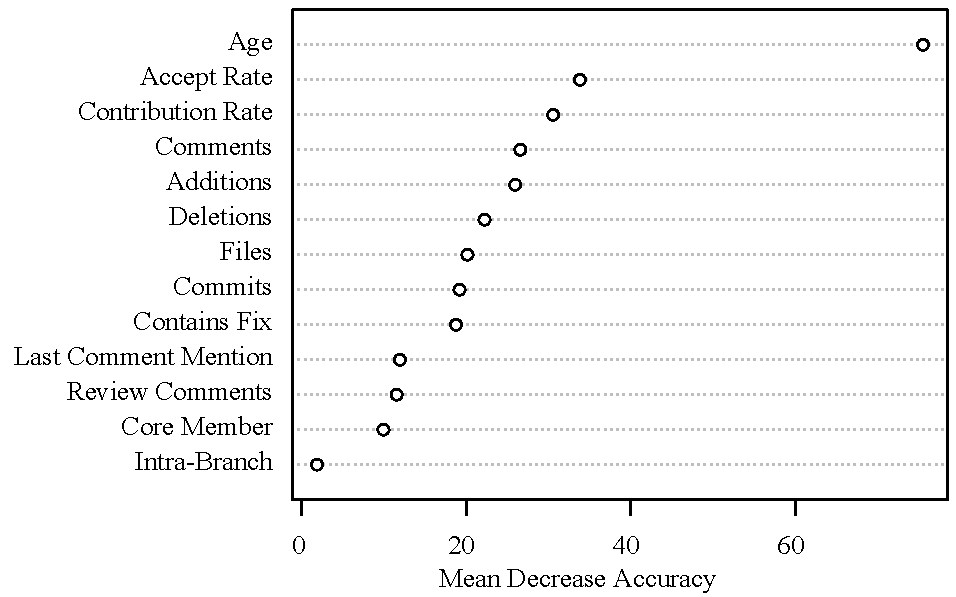
\includegraphics[width=0.45\textwidth]{../figs/mean-decrease-accuracy.pdf}
  \caption[Plot of feature importance]
   {Plot of feature importance. The age of the pull request is the dominant factor.}
  \label{fig:feature-importance}
\end{figure}

Again the feature selection didn't improve the performance of the Random Forest algorithm.
The results are shown in table~\ref{tab:feature-selection}.
Without the age feature the recall is less than with the feature.

\begin{table}
  \begin{tabular}{ l | c | c | c | c | c | c }
    Without & $\overline{p}$ & $\sigma(p)$ & $\overline{r}$ & $\sigma(r)$ & $\overline{F1}$ & $\sigma(F1)$ \\ \hline
    \hline
    Age & .6853 & .1079 & .4256 & .1647 & .5114 & .1463 \\
  \end{tabular}
  \caption[Feature selection]{Feature selection. The average precision, recall and F1-score for a model without some features. }
  \label{tab:feature-selection}
\end{table}

Despite the fact that it should be possible to further improve the prediction model and because this is only a preliminary study to prioritizing pull requests, we decided to go forward with the current model.

\subsection{Evaluation}
\label{sec:evaluation}

\erik{Discuss questionnaire here.}
